\section{Implementation}
\label{sec:implementation}
\begin{figure}[tb]\centering
  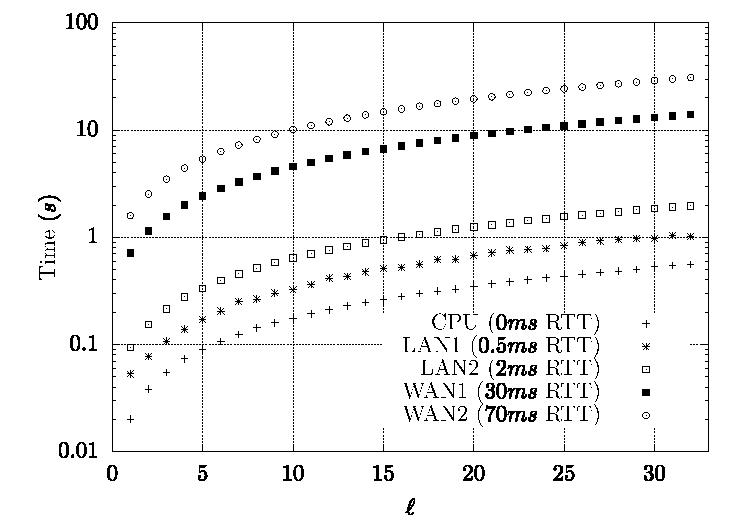
\includegraphics[width=\columnwidth]{plot.pdf}
  %\vspace*{-5mm}
  \caption{\label{figure}Total runtime of Construction~\ref{const:ioprf}}
\end{figure}
  \begin{table}[bb]\sisetup{detect-weight,mode=text}\small
    \centering\caption{\label{tab:imp}Cost breakdown}
    \sisetup{detect-weight,mode=text}
  \begin{tabular}{|c|cc|S[table-format=2.1]S[table-format=3.1]|cc|}
  \hline\multirow{2}{*}{$\ell$}& \multicolumn{2}{c|}{CPU (ms)}&\multicolumn{2}{c|}{Communication (kB)}&\multicolumn{2}{c|}{Total runtime (ms)}
  \\& Sender& Receiver & \multicolumn{1}{c}{Sender} & \multicolumn{1}{c|}{Receiver}& LAN1& WAN1
  \\\hline 5&44&41&11.7&26.1&171&2425
  \\10&88&81&23.2&51.4&325&4571
  \\15&126&123&34.6&76.6&512&6707
  \\20&174&162&46.1&101.9&679&8873
  \\25&218&202&57.5&127.1&836&10987
  \\30&267&248&69.0&152.4&968&13128
  \\\hline
\end{tabular}
\end{table}

To show practicality of Construction~\ref{const:ioprf} including its
ZK proofs, we have implemented and benchmarked its performance in
several realistic network settings. We stress that our implementation
is a full implementation of Construction~\ref{const:ioprf}, with all
Zero-Knowledge Proofs of Knowledge of Appendix~\ref{sec:sec-analysis},
i.e., including witness extractability and security against fully
malicious verifiers. Sender and receiver instances communicate via
standard TCP sockets.

Our implementation is done in $C$ and uses OpenSSL for elliptic curve
operations on NIST curve {\texttt{secp224r1}}. The source code is
available for download~\cite{srcode}.  We benchmark our implementation
on a 4.1~GHz Core i5-10600k.  As network latency is typically the
bottleneck in multi-round secure two-party computation protocols, we
benchmark Construction~\ref{const:ioprf} in different settings with
different network latencies.  To precisely control network latency
between sender and receiver instances, we use Linux' standard
{\texttt{tc-netem}} tool. Figure~\ref{figure} shows benchmark results
averaged over 50 executions, and Table~\ref{tab:imp} presents the cost
breakdown.

We measure total run time for values of $\ell$ ranging from $1$ to
$32$. Note that $\ell=32$ would support binary tree data structures
with $2^{32}$ different paths and $2^{33}-1$
(8.6~billion) nodes. We vary latency assuming LAN scenarios
with standard Gigabit Ethernet (0.5~ms RTT) or WiFi (2~ms RTT) and WAN
scenarios for intra-continental communication (30~ms RTT) and
inter-continental communication (70~ms RTT)~\cite{verizon}. We also
show an evaluation with 0~ms RTT, however even this number is still
dominated by the TCP communication overhead.  We found that the
computation alone in our protocol, including all EC computation and
ZKPs, is approximately 3~ms per $\ioprf$ iteration.

Each iOPRF evaluation for a tree data structure with $2^{20}$ nodes
needs about 170~ms of CPU time per party with our (unoptimized)
implementation.  As soon as we introduce higher latency, CPU time
contributes little to total runtime, and communication latency
becomes the main performance obstacle. For example, in the WAN1
scenario with intra-continental communication between sender and
receiver, total runtime is about 9~s of which less than $4\%$ is spent
with computation, and the remainder is consumed by network
latency.

We conclude from Figure~\ref{figure} that even for large values of
$\ell$ and for high latency network connections,
Construction~\ref{const:ioprf} has only a few seconds of runtime which
is practical for many scenarios.

In Appendix~\ref{sec:perf-related}, we discuss why alternative
approaches to realize the $\ioprf$ functionality perform worse than Construction~\ref{const:ioprf}.
